% Options for packages loaded elsewhere
\PassOptionsToPackage{unicode}{hyperref}
\PassOptionsToPackage{hyphens}{url}
%
\documentclass[
]{article}
\title{ARE 213 PS 3}
\author{S. Sung, H. Husain, T. Woolley, A. Watt}
\date{2021-12-8}

\usepackage{amsmath,amssymb}
\usepackage{lmodern}
\usepackage{iftex}
\ifPDFTeX
  \usepackage[T1]{fontenc}
  \usepackage[utf8]{inputenc}
  \usepackage{textcomp} % provide euro and other symbols
\else % if luatex or xetex
  \usepackage{unicode-math}
  \defaultfontfeatures{Scale=MatchLowercase}
  \defaultfontfeatures[\rmfamily]{Ligatures=TeX,Scale=1}
\fi
% Use upquote if available, for straight quotes in verbatim environments
\IfFileExists{upquote.sty}{\usepackage{upquote}}{}
\IfFileExists{microtype.sty}{% use microtype if available
  \usepackage[]{microtype}
  \UseMicrotypeSet[protrusion]{basicmath} % disable protrusion for tt fonts
}{}
\makeatletter
\@ifundefined{KOMAClassName}{% if non-KOMA class
  \IfFileExists{parskip.sty}{%
    \usepackage{parskip}
  }{% else
    \setlength{\parindent}{0pt}
    \setlength{\parskip}{6pt plus 2pt minus 1pt}}
}{% if KOMA class
  \KOMAoptions{parskip=half}}
\makeatother
\usepackage{xcolor}
\IfFileExists{xurl.sty}{\usepackage{xurl}}{} % add URL line breaks if available
\IfFileExists{bookmark.sty}{\usepackage{bookmark}}{\usepackage{hyperref}}
\hypersetup{
  pdftitle={ARE 213 PS 3},
  pdfauthor={S. Sung, H. Husain, T. Woolley, A. Watt},
  hidelinks,
  pdfcreator={LaTeX via pandoc}}
\urlstyle{same} % disable monospaced font for URLs
\usepackage[margin=1in]{geometry}
\usepackage{color}
\usepackage{fancyvrb}
\newcommand{\VerbBar}{|}
\newcommand{\VERB}{\Verb[commandchars=\\\{\}]}
\DefineVerbatimEnvironment{Highlighting}{Verbatim}{commandchars=\\\{\}}
% Add ',fontsize=\small' for more characters per line
\usepackage{framed}
\definecolor{shadecolor}{RGB}{248,248,248}
\newenvironment{Shaded}{\begin{snugshade}}{\end{snugshade}}
\newcommand{\AlertTok}[1]{\textcolor[rgb]{0.94,0.16,0.16}{#1}}
\newcommand{\AnnotationTok}[1]{\textcolor[rgb]{0.56,0.35,0.01}{\textbf{\textit{#1}}}}
\newcommand{\AttributeTok}[1]{\textcolor[rgb]{0.77,0.63,0.00}{#1}}
\newcommand{\BaseNTok}[1]{\textcolor[rgb]{0.00,0.00,0.81}{#1}}
\newcommand{\BuiltInTok}[1]{#1}
\newcommand{\CharTok}[1]{\textcolor[rgb]{0.31,0.60,0.02}{#1}}
\newcommand{\CommentTok}[1]{\textcolor[rgb]{0.56,0.35,0.01}{\textit{#1}}}
\newcommand{\CommentVarTok}[1]{\textcolor[rgb]{0.56,0.35,0.01}{\textbf{\textit{#1}}}}
\newcommand{\ConstantTok}[1]{\textcolor[rgb]{0.00,0.00,0.00}{#1}}
\newcommand{\ControlFlowTok}[1]{\textcolor[rgb]{0.13,0.29,0.53}{\textbf{#1}}}
\newcommand{\DataTypeTok}[1]{\textcolor[rgb]{0.13,0.29,0.53}{#1}}
\newcommand{\DecValTok}[1]{\textcolor[rgb]{0.00,0.00,0.81}{#1}}
\newcommand{\DocumentationTok}[1]{\textcolor[rgb]{0.56,0.35,0.01}{\textbf{\textit{#1}}}}
\newcommand{\ErrorTok}[1]{\textcolor[rgb]{0.64,0.00,0.00}{\textbf{#1}}}
\newcommand{\ExtensionTok}[1]{#1}
\newcommand{\FloatTok}[1]{\textcolor[rgb]{0.00,0.00,0.81}{#1}}
\newcommand{\FunctionTok}[1]{\textcolor[rgb]{0.00,0.00,0.00}{#1}}
\newcommand{\ImportTok}[1]{#1}
\newcommand{\InformationTok}[1]{\textcolor[rgb]{0.56,0.35,0.01}{\textbf{\textit{#1}}}}
\newcommand{\KeywordTok}[1]{\textcolor[rgb]{0.13,0.29,0.53}{\textbf{#1}}}
\newcommand{\NormalTok}[1]{#1}
\newcommand{\OperatorTok}[1]{\textcolor[rgb]{0.81,0.36,0.00}{\textbf{#1}}}
\newcommand{\OtherTok}[1]{\textcolor[rgb]{0.56,0.35,0.01}{#1}}
\newcommand{\PreprocessorTok}[1]{\textcolor[rgb]{0.56,0.35,0.01}{\textit{#1}}}
\newcommand{\RegionMarkerTok}[1]{#1}
\newcommand{\SpecialCharTok}[1]{\textcolor[rgb]{0.00,0.00,0.00}{#1}}
\newcommand{\SpecialStringTok}[1]{\textcolor[rgb]{0.31,0.60,0.02}{#1}}
\newcommand{\StringTok}[1]{\textcolor[rgb]{0.31,0.60,0.02}{#1}}
\newcommand{\VariableTok}[1]{\textcolor[rgb]{0.00,0.00,0.00}{#1}}
\newcommand{\VerbatimStringTok}[1]{\textcolor[rgb]{0.31,0.60,0.02}{#1}}
\newcommand{\WarningTok}[1]{\textcolor[rgb]{0.56,0.35,0.01}{\textbf{\textit{#1}}}}
\usepackage{graphicx}
\makeatletter
\def\maxwidth{\ifdim\Gin@nat@width>\linewidth\linewidth\else\Gin@nat@width\fi}
\def\maxheight{\ifdim\Gin@nat@height>\textheight\textheight\else\Gin@nat@height\fi}
\makeatother
% Scale images if necessary, so that they will not overflow the page
% margins by default, and it is still possible to overwrite the defaults
% using explicit options in \includegraphics[width, height, ...]{}
\setkeys{Gin}{width=\maxwidth,height=\maxheight,keepaspectratio}
% Set default figure placement to htbp
\makeatletter
\def\fps@figure{htbp}
\makeatother
\setlength{\emergencystretch}{3em} % prevent overfull lines
\providecommand{\tightlist}{%
  \setlength{\itemsep}{0pt}\setlength{\parskip}{0pt}}
\setcounter{secnumdepth}{-\maxdimen} % remove section numbering
\usepackage{dcolumn}
\usepackage{amsmath}
\usepackage{booktabs}
\usepackage{longtable}
\usepackage{array}
\usepackage{multirow}
\usepackage{wrapfig}
\usepackage{float}
\usepackage{colortbl}
\usepackage{pdflscape}
\usepackage{tabu}
\usepackage{threeparttable}
\usepackage{threeparttablex}
\usepackage[normalem]{ulem}
\usepackage{makecell}
\usepackage{xcolor}
\ifLuaTeX
  \usepackage{selnolig}  % disable illegal ligatures
\fi

\begin{document}
\maketitle

\newpage

\hypertarget{problem-1}{%
\section{Problem 1}\label{problem-1}}

\textbf{This question asks you to run OLS regressions that look at
whether there is an association between 2000 housing values and whether
a census tract contained a hazardous waste site that was placed on the
NPL by 2000.}

\hypertarget{part-a}{%
\subsection{Part (a)}\label{part-a}}

\textbf{Use the file allsites.dta. This file contains only own tract
housing variables (i.e.~no 2 mile averages). Use ``robust'' standard
errors for all regressions. First regress 2000 housing prices on whether
the census tract had an NPL site in 2000. Include 1980 housing values as
a control. Next add housing characteristics as controls. Run a third
regression adding economic and demographic variables as controls.
Finally run a 4th regression that also includes state fixed effects.
Briefly interpret the regressions. Under what conditions will the
coeffcients on NPL 2000 status be unbiased?}

\begin{verbatim}
## 
## =================================================================
##                                  Dependent variable:             
##                     ---------------------------------------------
##                                                lnmdvalhs0
##                            coefficient           felm  
##                                test                    
##                       (1)      (2)      (3)           (4)        
## -----------------------------------------------------------------
## npl2000             0.033*** 0.034*** 0.068***      0.063***     
##                     (0.013)  (0.012)  (0.010)       (0.009)      
##                                                                  
## -----------------------------------------------------------------
## Observations                                         42,881      
## R2                                                   0.779       
## Adjusted R2                                          0.779       
## Residual Std. Error                            0.294 (df = 42793)
## =================================================================
## Note:                                 *p<0.1; **p<0.05; ***p<0.01
\end{verbatim}

First, note that before starting Q1, we observed duplicate observations
in `allsite.dta'. These duplicates were dropped.

Second, we can see that coefficient on NPL2000 was statistically
significant under all four specifications.

In order to be consistent and unbiased, we need NPL2000 to be randomly
assigned (or as good as random given controls for more complex model
specifications) and that there exists no correlation between NPL2000 and
2000 Housing Price via unobservable factor, which would thereby be
captured through an error term.

\newpage

\hypertarget{part-b}{%
\subsection{Part (b)}\label{part-b}}

\textbf{Here we will compare covariates between potential treatment and
comparison groups. First, use allcovariates.dta to compare co-variates
(i.e.~those used in the above regressions) between census tracts with
and without a hazardous waste site listed on the NPL by 2000. Next, use
sitecovariates.dta to compare covariates between those census tracts
with a hazardous waste site that had an HRS test in 1982. Specifically,
compare those with sites that scored above 28.5 to those that scored
below 28.5. Finally, compare those census tracts with sites between 16.5
and 28.5 to census tracts with sites between 28.5 and 40.5. What
conclusions do you draw from these 3 comparisons?}

\begin{verbatim}
##            variable p_val_sp1 t_val_sp1 p_val_sp2 t_val_sp2 p_val_sp3 t_val_sp3
## 1       attach80occ     0.000    -9.089     0.041    -2.056     0.298    -1.044
## 2           avhhin8     0.000    -5.395     0.013     2.493     0.486     0.698
## 3     ba_or_better8     0.000   -10.898     0.000     4.915     0.036     2.114
## 4     bedrms0_80occ     0.047    -1.991     0.458     0.742     0.641     0.467
## 5     bedrms1_80occ     0.063    -1.863     0.617    -0.500     0.897    -0.130
## 6     bedrms2_80occ     0.001     3.376     0.001    -3.354     0.041    -2.057
## 7     bedrms3_80occ     0.490     0.690     0.636     0.474     0.472     0.721
## 8     bedrms4_80occ     0.004    -2.858     0.000     4.106     0.089     1.707
## 9     bedrms5_80occ     0.000    -4.184     0.010     2.574     0.219     1.232
## 10   blt0_1yrs80occ     0.004    -2.873     0.042     2.035     0.960     0.051
## 11 blt10_20yrs80occ     0.033     2.136     0.025     2.248     0.687     0.404
## 12   blt2_5yrs80occ     0.517     0.649     0.116     1.574     0.994    -0.008
## 13 blt20_30yrs80occ     0.114     1.581     0.520     0.643     0.961     0.049
## 14 blt30_40yrs80occ     0.811     0.239     0.060    -1.884     0.481    -0.707
## 15   blt40_yrs80occ     0.000    -4.098     0.007    -2.705     0.896    -0.130
## 16  blt6_10yrs80occ     0.000     3.885     0.018     2.381     0.649     0.456
## 17           child8     0.000     7.771     0.958     0.053     0.568     0.571
## 18      detach80occ     0.556    -0.589     0.050     1.968     0.108     1.618
## 19             ffh8     0.000    -6.931     0.018    -2.389     0.862     0.174
## 20  firestoveheat80     0.000     4.267     0.814    -0.236     0.510    -0.660
## 21          hsdrop8     0.623     0.492     0.235    -1.189     0.303    -1.033
## 22      mobile80occ     0.000     8.832     0.793    -0.263     0.285    -1.072
## 23   no_hs_diploma8     0.000     5.697     0.000    -4.679     0.060    -1.890
## 24      noaircond80     0.000     7.598     0.253    -1.145     0.870    -0.164
## 25  nofullkitchen80     0.089     1.701     0.402    -0.839     0.787    -0.271
## 26       occupied80     0.000     4.570     0.940     0.076     0.989    -0.014
## 27          ownocc8     0.000     7.040     0.922    -0.098     0.244    -1.169
## 28         pop_den8     0.000   -44.804     0.068    -1.833     0.571    -0.568
## 29          povrat8     0.044    -2.018     0.109    -1.606     0.716     0.364
## 30          shrblk8     0.000    -3.666     0.037    -2.095     0.926     0.093
## 31          shrfor8     0.000    -6.628     0.735    -0.339     0.785    -0.273
## 32          shrhsp8     0.000    -5.288     0.841    -0.201     0.928    -0.090
## 33           smhse8     0.000     6.358     0.001    -3.283     0.244    -1.168
## 34         tothsun8     0.029     2.187     0.951    -0.062     0.576    -0.561
## 35         unemprt8     0.005     2.832     0.001    -3.386     0.731    -0.345
## 36         welfare8     0.239    -1.178     0.041    -2.050     0.578    -0.557
## 37   zerofullbath80     0.009     2.625     0.089    -1.704     0.386    -0.868
\end{verbatim}

In the table (technically saved in dataframe format), we check for
balance of covariates (same ones used in 1(a)) across three potential
treatment and control groups. In the first specification, treatment
group is tracts on NPL list by 2000 and control is the counterpart. In
the corresponding column 1 and 2, we can see that means are
statistically significantly different on most variables across the two
groups. In the second specification, treatment group is census tracts
with HRS score in 1982 above 28.5 and control goups is census tracts
with score below 28.5. And the tracts without HRS testing in 1982 are
omitted. Comparing across 37 covariates, we can again see that on 16
covariates there is statistically significant difference between the two
groups. In the final specification, we get closer to treatment and
control groups we would use in Regression Discontinuity design. We can
see that p\_values are significantly larger and we seeem to observe
balance across most covariates. Hence, except for which tracts were
placed on NPL list or not, the two groups look similar on average on
observable dimensions.

\includegraphics{ps3_files/figure-latex/Love plot for NPL2000-1.pdf}

\begin{table}[!htbp] \centering 
  \caption{} 
  \label{} 
\begin{tabular}{@{\extracolsep{5pt}}lcccc} 
\\[-1.8ex]\hline 
\hline \\[-1.8ex] 
Statistic & \multicolumn{1}{c}{N} & \multicolumn{1}{c}{Mean} & \multicolumn{1}{c}{Min} & \multicolumn{1}{c}{Max} \\ 
\hline \\[-1.8ex] 
npl2000 & 48,176 & 0.019 & 0 & 1 \\ 
\hline \\[-1.8ex] 
\end{tabular} 
\end{table}

\hypertarget{section}{%
\section[]{\texorpdfstring{\protect\includegraphics{ps3_files/figure-latex/Love plot for HRS test in 1982 geq 28.5-1.pdf}}{}}\label{section}}

\hypertarget{statistic-n-mean-min-max}{%
\subsection{Statistic N Mean Min Max}\label{statistic-n-mean-min-max}}

\hypertarget{treat-487-0.628-0-1}{%
\subsection{treat 487 0.628 0 1}\label{treat-487-0.628-0-1}}

\hypertarget{section-1}{%
\section[]{\texorpdfstring{\protect\includegraphics{ps3_files/figure-latex/Love plot for HRS test in 1982 geq 28.5 between 16.5 and 40.5-1.pdf}}{}}\label{section-1}}

\hypertarget{statistic-n-mean-min-max-1}{%
\subsection{Statistic N Mean Min Max}\label{statistic-n-mean-min-max-1}}

\hypertarget{treat-227-0.604-0-1}{%
\subsection{treat 227 0.604 0 1}\label{treat-227-0.604-0-1}}

The three love plots above graphically depict the standardized
difference of means and variance ratios between the NPL2000 groups. The
rule of thumb is a standardized difference of means smaller than 0.25 in
magnitude, ideally less than 0.1 and as close to 0 as possible. The rule
of thumb for variance ratios is less than a factor of 2 (so between 0.5
and 2 in magnitude).

The first love plot is comparing the census tracts with and without a
hazardous waste site listed on the NPL by 2000 (48,176 sites total, with
1.9\% of them on the NPL). The second love plot comparing census tracts
with a hazardous waste site that had an HRS test in 1982, above and
below the 28.5 threshold (which is a significant reduction in sample
size: 487 tracts with 62.8\% above the threshold). We can see the
difference in means and variance ratios for all our variables are
getting closer to the rule of thumb above.

The last love plot has census tracts with a hazardous waste site that
had an HRS test in 1982 with an HRS score between 16.5 and 40.5,
comparing tracts above and below the 28.5 threshold. This further
restricts the sample to 227 tracts with 60.4\% above the threshold. The
standardized difference of means are not substantially different from
the second plot but the variance ratios have gotten worse for some of
our covariates.

\newpage

\hypertarget{problem-2}{%
\section{Problem 2}\label{problem-2}}

\textbf{This question examines the possibility of using a Regression
Discontinuity research design. Note that the rest of the empirical
question will use the file 2miledata.dta. The housing variables in this
file are 2 mile averages.}

\hypertarget{part-a-1}{%
\subsection{Part (a)}\label{part-a-1}}

\textbf{Consider the HRS score as the running variable for an RD
research design. What assumptions are needed on the HRS score? How do
each of the following ``facts'' impact the appropriateness of these
assumptions:}

The assumptions we need to hold for a cutoff to be useful in an RD
setting are that (1) The probability of treatment (NPL) should change
discontinuously at the threshold of running variable (HRS). (2) We
should not see bunching around the threshold, which may be indicative of
manipulation in treatment status.

Assumption (1) is not an huge issue in this setting since the cutoff was
strict in one direction. The fact that is is not strict in the other
direction, however, makes us think it could be a slight concern. The
following could either support assumption (2) or call it into question.

\hypertarget{a.i}{%
\subsubsection{------ a.i}\label{a.i}}

\textbf{The EPA assertion that the 28.5 cutoff was selected because it
produced a manageable number of sites.'' }

This might cause one to question assumption (2) because it introduces a
sense that 28.5 was chosen intentionally rather than at random. Imagine,
for instance, that if the regulators are selecting the cutoff based on
manageability, then the regulators might line up all of the projects by
their scores and determine the cutoff at a cleanup-cost discontinuity.

\hypertarget{a.ii}{%
\subsubsection{------ a.ii}\label{a.ii}}

\textbf{None of the individuals involved in identifying the site,
testing the level of pollution, or running the 1982 HRS test knew the
cutoff threshold score. }

If true, then the data were not gathered with any knowledge of the
cutoff ex ante, which make assumption (2) a little more likely to hold.

\hypertarget{a.iii}{%
\subsubsection{------ a.iii}\label{a.iii}}

\textbf{EPA documentation emphasizes that the HRS test is an imperfect
scoring measure. }

If the HRS test is an imperfect measure, then this also supports
assumption (2). The more imperfect HRS is, the more comparable are the
treated and untreated groups and therefore the more ``randomly'' the
threshold is likely to have been assigned.

\newpage

\hypertarget{part-b-1}{%
\subsection{Part (b)}\label{part-b-1}}

\textbf{Create a histogram of the distribution (i.e.~density) of the
1982 HRS scores by dividing the HRS score into non-overlapping bins.
Include a vertical line at 28.5. Next, run local linear regressions on
either side of 28.5 using the midpoints of the bins as the data. What do
you conclude?}

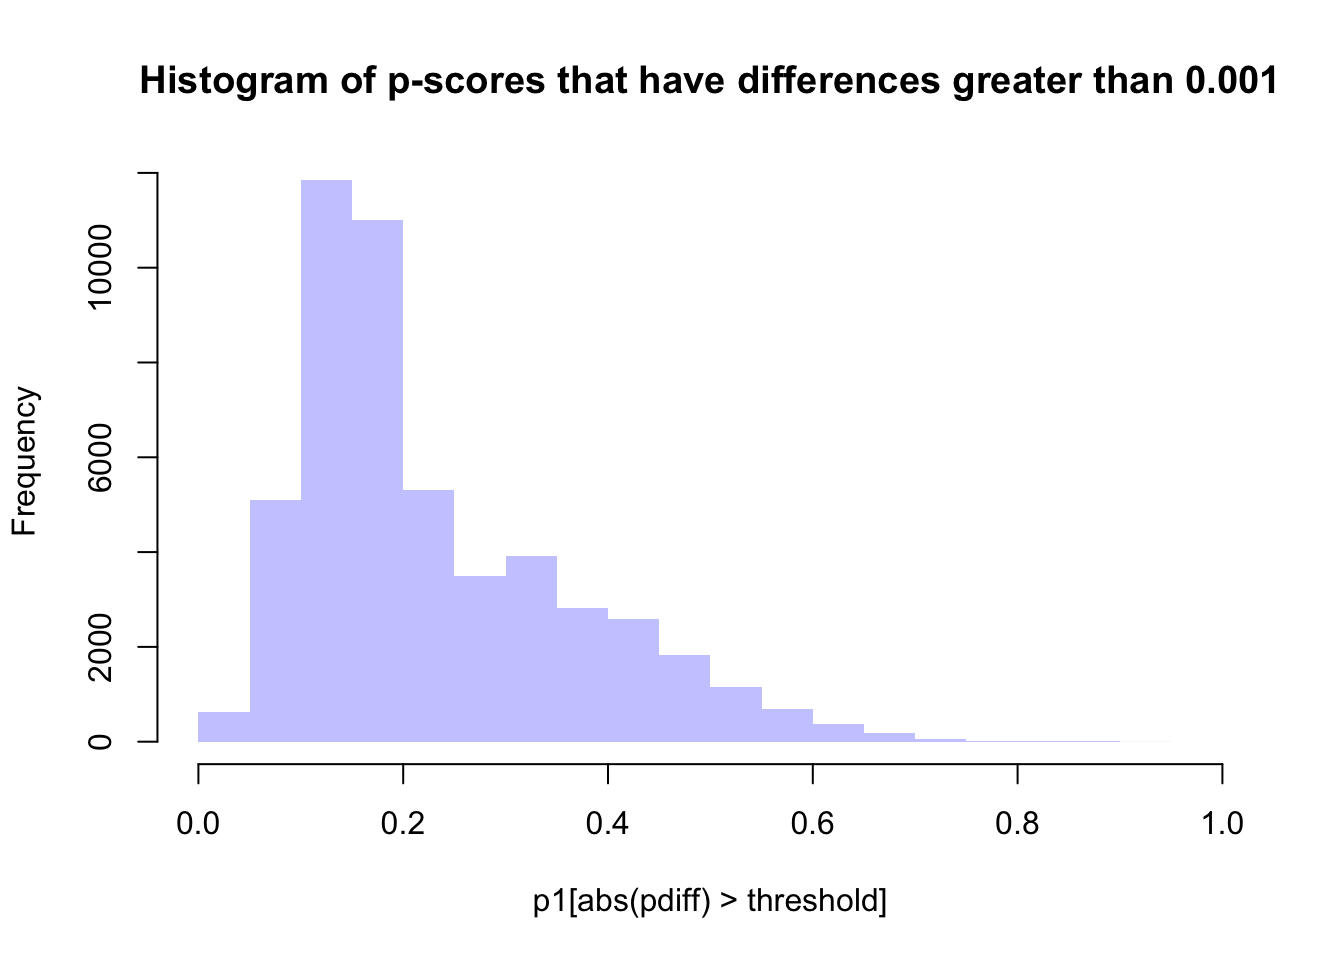
\includegraphics{ps3_files/figure-latex/unnamed-chunk-2-1.pdf}
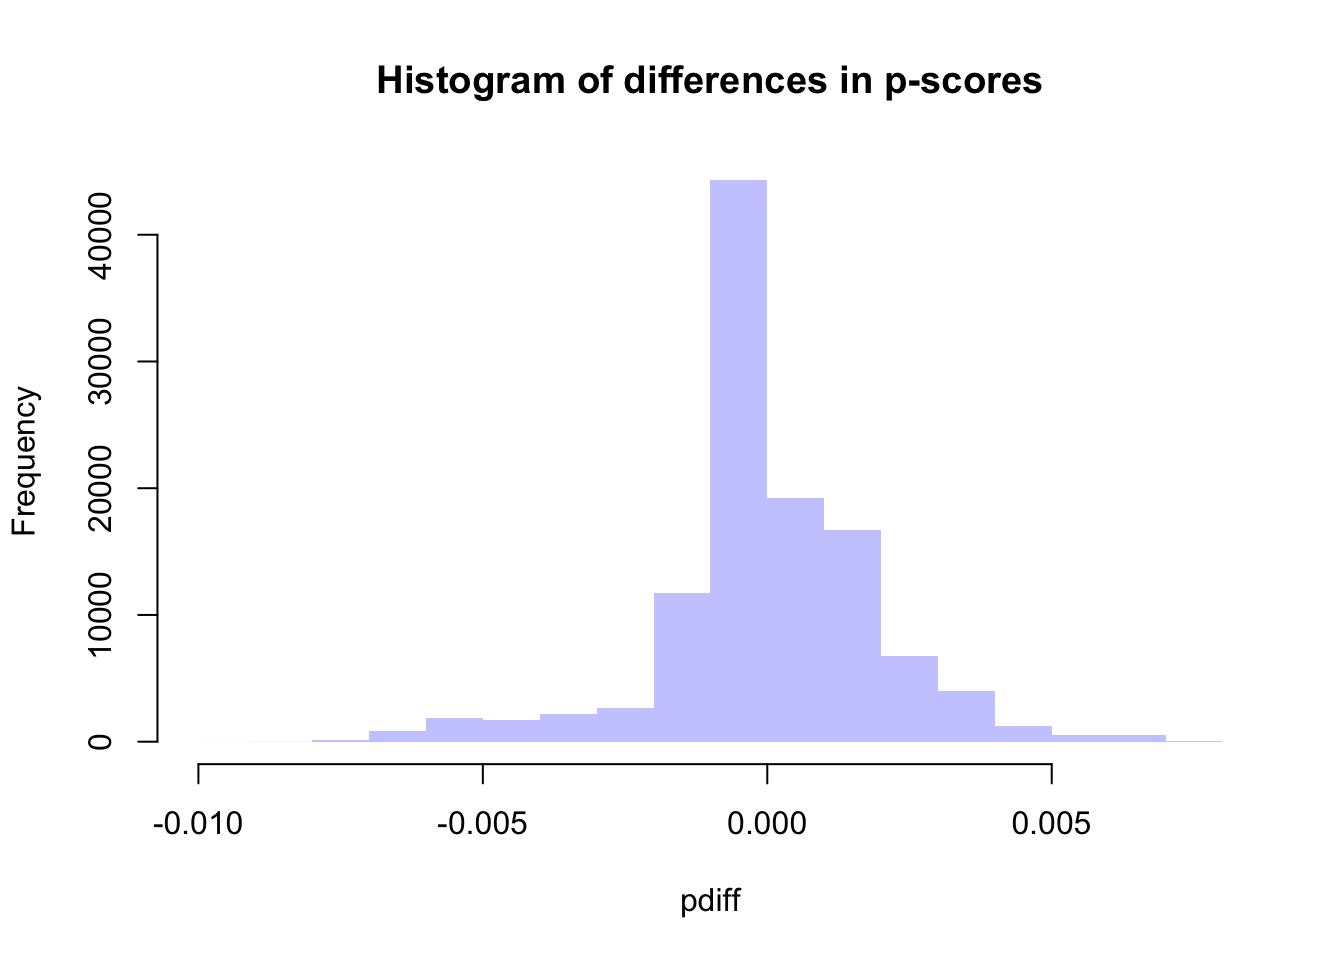
\includegraphics{ps3_files/figure-latex/unnamed-chunk-2-2.pdf}

\begin{verbatim}
## integer(0)
\end{verbatim}

\includegraphics{ps3_files/figure-latex/Plot narrower local linear regressions-1.pdf}
In the first histogram, there seems to be difference between regression
intercepts. However, in the second histogram, when we restrict the local
regressions to only include histogram bars closer to the threshold
(including 16.5 to 40.5), the difference between the regression
intercepts seems to disappear. The confidence intervals also show that
there is no discontinuity in the density of HRS scores at the HRS score
threshold, which suggests that there was no gaming of the system. This
makes the RD design more credible in the restricted sample.

\newpage

\hypertarget{problem-3}{%
\section{Problem 3}\label{problem-3}}

\textbf{This question examines the 1st stage equation of an RD design
using the 1982 HRS score.}

\hypertarget{part-a-2}{%
\subsection{Part (a)}\label{part-a-2}}

\textbf{Use a 2SLS (IV) econometric setup that uses whether or not a
census tract has a site scoring above/below 28.5 as the instrument.
Write down the 1st stage equation. Run the 1st stage regression
experimenting with the same set of covariates used in question (1). In
addition, run a second specification in which you limit the sample to
only those census tracts with sites between 16.5 and 40.5 and run the
specification using all of the control variables (we will use this as
the size of the bandwidth for the ``regression discontinuity''
regression). Interpret the results.}

Equations for 2SLS Set Up 1st Stage: \[
NPL2000_{i,s} = \alpha_1 + \beta_{1,1} 1(HRS1982 > 28.5)_i + \beta_{1,2} Covariates_{i} + \beta_{1,3} \theta_s + v_{i,s} 
\] 2nd Stage: \[
HousingPrice2000_{i,s} = \alpha_2 + \beta_{2,1} \hat{NPL_{i,2000}} + \beta_{2,2} Covariates_{i} + \beta_{2,3} \theta_s + \epsilon_{i,s}
\] Note: \(\theta_s\) is state fixed effects.

\begin{verbatim}
## 
## =====================================================
##                            Dependent variable:       
##                     ---------------------------------
##                                  npl2000             
##                           (1)              (2)       
## -----------------------------------------------------
## ind_hrsabove            0.799***         0.703***    
##                         (0.034)          (0.054)     
##                                                      
## -----------------------------------------------------
## Observations              483              226       
## R2                       0.797            0.705      
## Adjusted R2              0.759            0.566      
## Residual Std. Error 0.228 (df = 407) 0.301 (df = 153)
## =====================================================
## Note:                     *p<0.1; **p<0.05; ***p<0.01
\end{verbatim}

From this, we can conclude that NPL2000 is extremely predictive in the
first stage! This implies that we were wise to use the IV approach
before running the second stage reduced form.

\hypertarget{part-b-2}{%
\subsection{Part (b)}\label{part-b-2}}

\textbf{Create a graph plotting the the 1982 HRS score against whether a
site is listed on the NPL by year 2000 (NPL on the y-axis, HRS on the x
-axis). Briefly explain and interpret this graph.}

\includegraphics{ps3_files/figure-latex/unnamed-chunk-4-1.pdf}

Above graph demonstrates that we have a clear break at threshold but the
cut-off is not as perfect for strict RD design. Rather, we may want to
consider Fuzzy RD design. The few census tracts that has lower than 28.5
points on HRS score in 1982 measure but still manages to get on NPL by
2000 could perhaps (1) receive higher score on on HRS in proceeding
years, getting onto NPL before 2000, or (2) could potentially have other
reasons, i.e.~political connections or pressure, for getting onto the
list.

\hypertarget{part-c}{%
\subsection{Part (c)}\label{part-c}}

\textbf{Create a graph that plots the 1982 HRS score against 1980
property values (property values on the y-axis, HRS on the x -axis).
What do you conclude from this graph?}

\includegraphics{ps3_files/figure-latex/unnamed-chunk-5-1.pdf}

While median house price is definitely correlated with HRS score, it
seems to be continuous around the threshold and therefore satisfies our
assumptions for RD design.

\newpage

\hypertarget{problem-4}{%
\section{Problem 4}\label{problem-4}}

\textbf{Write down the 2nd stage equation (with housing values as the
out-come) and the 2 standard assumptions for valid IV estimation. Run
2SLS to get the estimated coefficient on 2000 NPL status. Run the same
two specifications as in the previous question. Briefly interpret the
results.}

Equations for 2SLS Set Up 1st Stage: \[
NPL2000_{i,s} = \alpha_1 + \beta_{1,1} 1(HRS1982 > 28.5)_i + \beta_{1,2} Covariates_{i} + \beta_{1,3} \theta_s + v_{i,s} 
\] 2nd Stage: \[
HousingPrice2000_{i,s} = \alpha_2 + \beta_{2,1} \hat{NPL_{i,2000}} + \beta_{2,2} Covariates_{i} + \beta_{2,3} \theta_s + \epsilon_{i,s}
\] Note: \(\theta_s\) is state fixed effects.

The standard assumptions for valid IV estimation is (1) Cov(HSR1982,
\epsilon\_\{i,s\}) = 0 and (2) Cov(HSR1982, NPL2000) =/= 0.

\begin{verbatim}
## 
## =====================================================
##                            Dependent variable:       
##                     ---------------------------------
##                                lnmdvalhs0            
##                           (1)              (2)       
## -----------------------------------------------------
## PredNPL                  -0.005           -0.001     
##                         (0.027)          (0.038)     
##                                                      
## -----------------------------------------------------
## Observations              483              226       
## R2                       0.851            0.889      
## Adjusted R2              0.823            0.836      
## Residual Std. Error 0.186 (df = 407) 0.171 (df = 153)
## =====================================================
## Note:                     *p<0.1; **p<0.05; ***p<0.01
\end{verbatim}

In the IV (2SLS) methods, both specification lead to statistically
insignificant coefficient. Hence, we observe that impact of being put on
NPL list by 2000 leads to little change in value of homes from 1980 to
2000.

\newpage

\hypertarget{problem-5}{%
\section{Problem 5}\label{problem-5}}

\textbf{Write a 1 paragraph conclusion summarizing your findings and
interpreting the results. Be sure to comment on how the evidence from
this problem set supports the primary research question.}

In the above 2SLS procedure, we find that being placed on NPL by year
2000 seems to have statistically insignificant impact on housing prices.
This would give interpretation that WTP or willingness to pay for
hazardous waste is very small. However, we should note there could be
additional factors why we get insignificant results. For example, if the
clean-up has not started in many sites by year 2,000 and clean-up
generally takes a long time, then not all the `benefits' or `willingness
to pay for clean-up' may have been internalized by year 2000. In this
case, running the analysis 10 years later with updated housing prices
may give different result. Alternatively, clean-up process may cause
negative externalities (i.e.~noise or trucks passing through) and
depress housing demand while in progress and perhaps after clean-up is
finished, given improved amenities, supply of housing increases. In any
of these cases, results could be measuring something slightly other than
Willingness to Pay for CleanUp.

\newpage

\hypertarget{appendix-a-r-code}{%
\section{Appendix A: R Code}\label{appendix-a-r-code}}

\begin{Shaded}
\begin{Highlighting}[]
\FunctionTok{rm}\NormalTok{(}\AttributeTok{list=}\FunctionTok{ls}\NormalTok{())}
\NormalTok{knitr}\SpecialCharTok{::}\NormalTok{opts\_chunk}\SpecialCharTok{$}\FunctionTok{set}\NormalTok{(}\AttributeTok{echo =}\NormalTok{ F, }\AttributeTok{warning =} \ConstantTok{FALSE}\NormalTok{, }\AttributeTok{message =} \ConstantTok{FALSE}\NormalTok{)}
\CommentTok{\# stargazer table type (html, latex, or text)}
\CommentTok{\# Change to latex when outputting to PDF, html when outputting to html}
\NormalTok{table\_type }\OtherTok{=} \StringTok{"latex"}
\FunctionTok{library}\NormalTok{(tidyverse)}
\FunctionTok{library}\NormalTok{(haven)}
\FunctionTok{library}\NormalTok{(stargazer)}
\FunctionTok{library}\NormalTok{(ggplot2)}
\FunctionTok{library}\NormalTok{(tinytex)}
\FunctionTok{library}\NormalTok{(lfe) }\CommentTok{\# For felm() fixed effects model}
\FunctionTok{library}\NormalTok{(lmtest)}
\FunctionTok{library}\NormalTok{(sandwich)}
\FunctionTok{library}\NormalTok{(cobalt)}
\FunctionTok{library}\NormalTok{(kableExtra)}
\NormalTok{allsite }\OtherTok{\textless{}{-}} \FunctionTok{read\_dta}\NormalTok{(}\StringTok{\textquotesingle{}allsites.dta\textquotesingle{}}\NormalTok{)}
\NormalTok{allcovariates }\OtherTok{\textless{}{-}} \FunctionTok{read\_dta}\NormalTok{(}\StringTok{\textquotesingle{}allcovariates.dta\textquotesingle{}}\NormalTok{)}
\NormalTok{twomiledata }\OtherTok{\textless{}{-}} \FunctionTok{read\_dta}\NormalTok{(}\StringTok{\textquotesingle{}2miledata.dta\textquotesingle{}}\NormalTok{)}
\NormalTok{sitecovariates }\OtherTok{\textless{}{-}} \FunctionTok{read\_dta}\NormalTok{(}\StringTok{\textquotesingle{}sitecovariates.dta\textquotesingle{}}\NormalTok{)}
\CommentTok{\# In "allsite.dta", we observe that there are duplicate observations. Dropped}
\FunctionTok{sum}\NormalTok{(}\FunctionTok{duplicated}\NormalTok{(allsite}\SpecialCharTok{$}\NormalTok{fips)) }\CommentTok{\# There are cases of duplicate observations with same FIPs.}
\FunctionTok{sum}\NormalTok{(}\FunctionTok{duplicated}\NormalTok{(allsite)) }\CommentTok{\# This confirms that their entire row values are }
                         \CommentTok{\# duplicates and can be dropped.}
\CommentTok{\# Duplicates Dropped for "allsite.dta"}
\NormalTok{allsite }\OtherTok{\textless{}{-}}\NormalTok{ allsite[}\SpecialCharTok{!}\FunctionTok{duplicated}\NormalTok{(allsite),]}

\CommentTok{\# Duplicates Dropped for "allcovarites.dta" {-} same procedure as above}
\FunctionTok{sum}\NormalTok{(}\FunctionTok{duplicated}\NormalTok{(allcovariates))}
\NormalTok{allcovariates }\OtherTok{\textless{}{-}}\NormalTok{ allcovariates[}\SpecialCharTok{!}\FunctionTok{duplicated}\NormalTok{(allcovariates),]}

\CommentTok{\# No duplicates in "twomiledata.dta"}
\FunctionTok{sum}\NormalTok{(}\FunctionTok{duplicated}\NormalTok{(twomiledata))}
\CommentTok{\# Regress 2000 housing prices on 1(NPL site in 2000) and 1980 housing values.}
\NormalTok{reg\_1a1 }\OtherTok{\textless{}{-}} \FunctionTok{lm}\NormalTok{(lnmdvalhs0 }\SpecialCharTok{\textasciitilde{}}\NormalTok{ npl2000 }\SpecialCharTok{+}\NormalTok{ lnmeanhs8, }\AttributeTok{data =}\NormalTok{ allsite)}
\NormalTok{reg\_1a1\_r }\OtherTok{\textless{}{-}} \FunctionTok{coeftest}\NormalTok{(reg\_1a1, }\AttributeTok{vcov =} \FunctionTok{vcovHC}\NormalTok{(reg\_1a1, }\AttributeTok{type =} \StringTok{"HC1"}\NormalTok{))}

\CommentTok{\# Regress: Add housing characteristics as control.}
\NormalTok{HousingChar }\OtherTok{\textless{}{-}} \FunctionTok{c}\NormalTok{(}\StringTok{"smhse8"}\NormalTok{, }\StringTok{"tothsun8"}\NormalTok{, }\StringTok{"ownocc8"}\NormalTok{, }\StringTok{"firestoveheat80"}\NormalTok{, }\StringTok{"noaircond80"}\NormalTok{, }
                 \StringTok{"nofullkitchen80"}\NormalTok{, }\StringTok{"zerofullbath80"}\NormalTok{, }
                \StringTok{"bedrms1\_80occ"}\NormalTok{, }\StringTok{"bedrms2\_80occ"}\NormalTok{, }\StringTok{"bedrms3\_80occ"}\NormalTok{, }\StringTok{"bedrms4\_80occ"}\NormalTok{, }\StringTok{"bedrms5\_80occ"}\NormalTok{,}
                \StringTok{"blt2\_5yrs80occ"}\NormalTok{, }\StringTok{"blt6\_10yrs80occ"}\NormalTok{, }\StringTok{"blt10\_20yrs80occ"}\NormalTok{, }\StringTok{"blt20\_30yrs80occ"}\NormalTok{, }\StringTok{"blt30\_40yrs80occ"}\NormalTok{, }\StringTok{"blt40\_yrs80occ"}\NormalTok{,}
                \StringTok{"detach80occ"}\NormalTok{, }\StringTok{"attach80occ"}\NormalTok{, }\StringTok{"mobile80occ"}\NormalTok{, }\StringTok{"occupied80"}\NormalTok{)}
\NormalTok{Formula1 }\OtherTok{\textless{}{-}} \FunctionTok{formula}\NormalTok{(}\FunctionTok{paste}\NormalTok{(}\StringTok{"lnmdvalhs0 \textasciitilde{} npl2000 + lnmeanhs8 + "}\NormalTok{, }\FunctionTok{paste}\NormalTok{(HousingChar, }\AttributeTok{collapse=}\StringTok{" + "}\NormalTok{)))}
\NormalTok{reg\_1a2 }\OtherTok{\textless{}{-}} \FunctionTok{lm}\NormalTok{(Formula1, }\AttributeTok{data =}\NormalTok{ allsite)}
\NormalTok{reg\_1a2\_r }\OtherTok{\textless{}{-}} \FunctionTok{coeftest}\NormalTok{(reg\_1a2, }\AttributeTok{vcov =} \FunctionTok{vcovHC}\NormalTok{(reg\_1a2, }\AttributeTok{type =} \StringTok{"HC1"}\NormalTok{))}

\CommentTok{\# Regress: Add economic and demographic variables as control.}
\NormalTok{EconNDemo }\OtherTok{\textless{}{-}} \FunctionTok{c}\NormalTok{(}\StringTok{"pop\_den8"}\NormalTok{, }\StringTok{"shrblk8"}\NormalTok{, }\StringTok{"shrhsp8"}\NormalTok{, }\StringTok{"child8"}\NormalTok{, }\StringTok{"old8"}\NormalTok{, }\StringTok{"shrfor8"}\NormalTok{, }\StringTok{"ffh8"}\NormalTok{, }
               \StringTok{"hsdrop8"}\NormalTok{, }\StringTok{"no\_hs\_diploma8"}\NormalTok{, }\StringTok{"ba\_or\_better8"}\NormalTok{, }\StringTok{"unemprt8"}\NormalTok{, }\StringTok{"povrat8"}\NormalTok{, }
               \StringTok{"welfare8"}\NormalTok{, }\StringTok{"avhhin8"}\NormalTok{)}
\NormalTok{Formula2 }\OtherTok{\textless{}{-}} \FunctionTok{formula}\NormalTok{(}\FunctionTok{paste}\NormalTok{(}\StringTok{"lnmdvalhs0 \textasciitilde{} npl2000 + lnmeanhs8 + "}\NormalTok{, }\FunctionTok{paste}\NormalTok{(}\FunctionTok{c}\NormalTok{(HousingChar, EconNDemo), }\AttributeTok{collapse=}\StringTok{" + "}\NormalTok{)))}
\NormalTok{reg\_1a3 }\OtherTok{\textless{}{-}} \FunctionTok{lm}\NormalTok{(Formula2, }\AttributeTok{data =}\NormalTok{ allsite)}
\NormalTok{reg\_1a3\_r }\OtherTok{\textless{}{-}} \FunctionTok{coeftest}\NormalTok{(reg\_1a3, }\AttributeTok{vcov =} \FunctionTok{vcovHC}\NormalTok{(reg\_1a3, }\AttributeTok{type =} \StringTok{"HC1"}\NormalTok{))}

\CommentTok{\# Include State FE}
\NormalTok{Formula3 }\OtherTok{\textless{}{-}} \FunctionTok{formula}\NormalTok{(}\FunctionTok{paste}\NormalTok{(}\StringTok{"lnmdvalhs0 \textasciitilde{} npl2000 + lnmeanhs8 + "}\NormalTok{, }\FunctionTok{paste}\NormalTok{(}\FunctionTok{c}\NormalTok{(HousingChar, EconNDemo), }\AttributeTok{collapse=}\StringTok{" + "}\NormalTok{), }\StringTok{" | statefips"}\NormalTok{))}
\NormalTok{reg\_1a4 }\OtherTok{\textless{}{-}} \FunctionTok{felm}\NormalTok{(Formula3, }\AttributeTok{data =}\NormalTok{ allsite)}

\CommentTok{\# Stargazer Table with All Four Regressions}
\FunctionTok{stargazer}\NormalTok{(reg\_1a1\_r, reg\_1a2\_r, reg\_1a3\_r, reg\_1a4,}
          \AttributeTok{se =} \FunctionTok{list}\NormalTok{(reg\_1a1\_r[,}\DecValTok{2}\NormalTok{], reg\_1a2\_r[,}\DecValTok{2}\NormalTok{], reg\_1a3\_r[,}\DecValTok{2}\NormalTok{], reg\_1a4}\SpecialCharTok{$}\NormalTok{rse),}
          \AttributeTok{keep =} \StringTok{"npl2000"}\NormalTok{, }\AttributeTok{type =} \StringTok{"text"}\NormalTok{, }\AttributeTok{omit.stat =} \StringTok{"f"}\NormalTok{)}
\CommentTok{\# Using "allcovariates.dta", compare covariates between treatment and comparison groups.}
\CommentTok{\# Note: variable "old8" is not available in "allcovariates.dta"}
\NormalTok{ttest\_1 }\OtherTok{\textless{}{-}}\NormalTok{ allcovariates }\SpecialCharTok{\%\textgreater{}\%}
                \FunctionTok{mutate}\NormalTok{(}\AttributeTok{npl2000\_f =} \FunctionTok{ifelse}\NormalTok{(npl2000 }\SpecialCharTok{==} \DecValTok{1}\NormalTok{, }\StringTok{"OnList"}\NormalTok{, }\StringTok{"NotOnList"}\NormalTok{)) }\SpecialCharTok{\%\textgreater{}\%}
                \FunctionTok{select}\NormalTok{(npl2000\_f, }
\NormalTok{                          smhse8, tothsun8, ownocc8, firestoveheat80, }
\NormalTok{                          noaircond80, nofullkitchen80, zerofullbath80, }
\NormalTok{                          bedrms0\_80occ, bedrms1\_80occ, bedrms2\_80occ, }
\NormalTok{                            bedrms3\_80occ, bedrms4\_80occ, bedrms5\_80occ,}
\NormalTok{                          blt0\_1yrs80occ, blt2\_5yrs80occ, blt6\_10yrs80occ, }
\NormalTok{                            blt10\_20yrs80occ, blt20\_30yrs80occ, blt30\_40yrs80occ, blt40\_yrs80occ,}
\NormalTok{                          detach80occ, attach80occ, mobile80occ, occupied80,}
\NormalTok{                          pop\_den8, shrblk8, shrhsp8, child8, shrfor8, ffh8,}
\NormalTok{                          hsdrop8, no\_hs\_diploma8, ba\_or\_better8, unemprt8, povrat8, }
\NormalTok{                          welfare8, avhhin8) }\SpecialCharTok{\%\textgreater{}\%}
                \FunctionTok{gather}\NormalTok{(}\AttributeTok{key =}\NormalTok{ variable, }\AttributeTok{value =}\NormalTok{ value, }\SpecialCharTok{{-}}\NormalTok{ npl2000\_f) }\SpecialCharTok{\%\textgreater{}\%}
                \FunctionTok{group\_by}\NormalTok{(npl2000\_f, variable) }\SpecialCharTok{\%\textgreater{}\%}
                \FunctionTok{summarise}\NormalTok{(}\AttributeTok{value =} \FunctionTok{list}\NormalTok{(value)) }\SpecialCharTok{\%\textgreater{}\%}
                \FunctionTok{spread}\NormalTok{(npl2000\_f, value) }\SpecialCharTok{\%\textgreater{}\%}
                \FunctionTok{group\_by}\NormalTok{(variable) }\SpecialCharTok{\%\textgreater{}\%}
                \FunctionTok{mutate}\NormalTok{(}\AttributeTok{p\_value =} \FunctionTok{t.test}\NormalTok{(}\FunctionTok{unlist}\NormalTok{(OnList), }\FunctionTok{unlist}\NormalTok{(NotOnList))}\SpecialCharTok{$}\NormalTok{p.value,}
                       \AttributeTok{t\_value =} \FunctionTok{t.test}\NormalTok{(}\FunctionTok{unlist}\NormalTok{(OnList), }\FunctionTok{unlist}\NormalTok{(NotOnList))}\SpecialCharTok{$}\NormalTok{statistic) }\SpecialCharTok{\%\textgreater{}\%}
                \FunctionTok{select}\NormalTok{(variable, p\_value, t\_value) }\SpecialCharTok{\%\textgreater{}\%}
                \FunctionTok{rename}\NormalTok{(}\AttributeTok{p\_val\_sp1 =}\NormalTok{ p\_value, }\AttributeTok{t\_val\_sp1 =}\NormalTok{ t\_value)}

\CommentTok{\# Using "sitecovariates.dta", compare covarites between census tracts with HRS test score from 1982 above and below 28.5.}
\CommentTok{\# Note: variable "old8" is not available in "allcovariates.dta"}
\NormalTok{ttest\_2 }\OtherTok{\textless{}{-}}\NormalTok{ sitecovariates }\SpecialCharTok{\%\textgreater{}\%}
                \FunctionTok{mutate}\NormalTok{(}\AttributeTok{above =} \FunctionTok{ifelse}\NormalTok{(hrs\_82 }\SpecialCharTok{\textgreater{}} \FloatTok{28.5}\NormalTok{, }\StringTok{"Above"}\NormalTok{, }\StringTok{"Below"}\NormalTok{)) }\SpecialCharTok{\%\textgreater{}\%}
                \FunctionTok{select}\NormalTok{(above, }
\NormalTok{                          smhse8, tothsun8, ownocc8, firestoveheat80, }
\NormalTok{                          noaircond80, nofullkitchen80, zerofullbath80, }
\NormalTok{                          bedrms0\_80occ, bedrms1\_80occ, bedrms2\_80occ, }
\NormalTok{                            bedrms3\_80occ, bedrms4\_80occ, bedrms5\_80occ,}
\NormalTok{                          blt0\_1yrs80occ, blt2\_5yrs80occ, blt6\_10yrs80occ, }
\NormalTok{                            blt10\_20yrs80occ, blt20\_30yrs80occ, blt30\_40yrs80occ, blt40\_yrs80occ,}
\NormalTok{                          detach80occ, attach80occ, mobile80occ, occupied80,}
\NormalTok{                          pop\_den8, shrblk8, shrhsp8, child8, shrfor8, ffh8,}
\NormalTok{                          hsdrop8, no\_hs\_diploma8, ba\_or\_better8, unemprt8, povrat8, }
\NormalTok{                          welfare8, avhhin8) }\SpecialCharTok{\%\textgreater{}\%}
                \FunctionTok{gather}\NormalTok{(}\AttributeTok{key =}\NormalTok{ variable, }\AttributeTok{value =}\NormalTok{ value, }\SpecialCharTok{{-}}\NormalTok{ above) }\SpecialCharTok{\%\textgreater{}\%}
                \FunctionTok{group\_by}\NormalTok{(above, variable) }\SpecialCharTok{\%\textgreater{}\%}
                \FunctionTok{summarise}\NormalTok{(}\AttributeTok{value =} \FunctionTok{list}\NormalTok{(value)) }\SpecialCharTok{\%\textgreater{}\%}
                \FunctionTok{spread}\NormalTok{(above, value) }\SpecialCharTok{\%\textgreater{}\%}
                \FunctionTok{group\_by}\NormalTok{(variable) }\SpecialCharTok{\%\textgreater{}\%}
                \FunctionTok{mutate}\NormalTok{(}\AttributeTok{p\_value =} \FunctionTok{t.test}\NormalTok{(}\FunctionTok{unlist}\NormalTok{(Above), }\FunctionTok{unlist}\NormalTok{(Below))}\SpecialCharTok{$}\NormalTok{p.value,}
                       \AttributeTok{t\_value =} \FunctionTok{t.test}\NormalTok{(}\FunctionTok{unlist}\NormalTok{(Above), }\FunctionTok{unlist}\NormalTok{(Below))}\SpecialCharTok{$}\NormalTok{statistic) }\SpecialCharTok{\%\textgreater{}\%}
                \FunctionTok{select}\NormalTok{(variable, p\_value, t\_value) }\SpecialCharTok{\%\textgreater{}\%}
                \FunctionTok{rename}\NormalTok{(}\AttributeTok{p\_val\_sp2 =}\NormalTok{ p\_value, }\AttributeTok{t\_val\_sp2 =}\NormalTok{ t\_value)}

\CommentTok{\# Using "sitecovaraites.dta", compare covarites between census tracts with HRS test score from 1982 of 28.5{-}40.5 and 16.5{-}28.5.}
\NormalTok{ttest\_3 }\OtherTok{\textless{}{-}}\NormalTok{ sitecovariates }\SpecialCharTok{\%\textgreater{}\%}
                \FunctionTok{filter}\NormalTok{(hrs\_82 }\SpecialCharTok{\textgreater{}=} \FloatTok{16.5} \SpecialCharTok{\&}\NormalTok{ hrs\_82 }\SpecialCharTok{\textless{}=} \FloatTok{40.5}\NormalTok{) }\SpecialCharTok{\%\textgreater{}\%}
                \FunctionTok{mutate}\NormalTok{(}\AttributeTok{justabove =} \FunctionTok{ifelse}\NormalTok{(hrs\_82 }\SpecialCharTok{\textgreater{}} \FloatTok{28.5}\NormalTok{, }\StringTok{"JustAbove"}\NormalTok{, }\StringTok{"JustBelow"}\NormalTok{)) }\SpecialCharTok{\%\textgreater{}\%}
                \FunctionTok{select}\NormalTok{(justabove, }
\NormalTok{                          smhse8, tothsun8, ownocc8, firestoveheat80, }
\NormalTok{                          noaircond80, nofullkitchen80, zerofullbath80, }
\NormalTok{                          bedrms0\_80occ, bedrms1\_80occ, bedrms2\_80occ, }
\NormalTok{                            bedrms3\_80occ, bedrms4\_80occ, bedrms5\_80occ,}
\NormalTok{                          blt0\_1yrs80occ, blt2\_5yrs80occ, blt6\_10yrs80occ, }
\NormalTok{                            blt10\_20yrs80occ, blt20\_30yrs80occ, blt30\_40yrs80occ, blt40\_yrs80occ,}
\NormalTok{                          detach80occ, attach80occ, mobile80occ, occupied80,}
\NormalTok{                          pop\_den8, shrblk8, shrhsp8, child8, shrfor8, ffh8,}
\NormalTok{                          hsdrop8, no\_hs\_diploma8, ba\_or\_better8, unemprt8, povrat8, }
\NormalTok{                          welfare8, avhhin8) }\SpecialCharTok{\%\textgreater{}\%}
                \FunctionTok{gather}\NormalTok{(}\AttributeTok{key =}\NormalTok{ variable, }\AttributeTok{value =}\NormalTok{ value, }\SpecialCharTok{{-}}\NormalTok{ justabove) }\SpecialCharTok{\%\textgreater{}\%}
                \FunctionTok{group\_by}\NormalTok{(justabove, variable) }\SpecialCharTok{\%\textgreater{}\%}
                \FunctionTok{summarise}\NormalTok{(}\AttributeTok{value =} \FunctionTok{list}\NormalTok{(value)) }\SpecialCharTok{\%\textgreater{}\%}
                \FunctionTok{spread}\NormalTok{(justabove, value) }\SpecialCharTok{\%\textgreater{}\%}
                \FunctionTok{group\_by}\NormalTok{(variable) }\SpecialCharTok{\%\textgreater{}\%}
                \FunctionTok{mutate}\NormalTok{(}\AttributeTok{p\_value =} \FunctionTok{t.test}\NormalTok{(}\FunctionTok{unlist}\NormalTok{(JustAbove), }\FunctionTok{unlist}\NormalTok{(JustBelow))}\SpecialCharTok{$}\NormalTok{p.value,}
                       \AttributeTok{t\_value =} \FunctionTok{t.test}\NormalTok{(}\FunctionTok{unlist}\NormalTok{(JustAbove), }\FunctionTok{unlist}\NormalTok{(JustBelow))}\SpecialCharTok{$}\NormalTok{statistic) }\SpecialCharTok{\%\textgreater{}\%}
                \FunctionTok{select}\NormalTok{(variable, p\_value, t\_value) }\SpecialCharTok{\%\textgreater{}\%}
                \FunctionTok{rename}\NormalTok{(}\AttributeTok{p\_val\_sp3 =}\NormalTok{ p\_value, }\AttributeTok{t\_val\_sp3 =}\NormalTok{ t\_value)}

\CommentTok{\# Output t{-}test results}
\NormalTok{merged }\OtherTok{\textless{}{-}} \FunctionTok{left\_join}\NormalTok{(ttest\_1, ttest\_2, }\AttributeTok{by =} \StringTok{\textquotesingle{}variable\textquotesingle{}}\NormalTok{)}
\NormalTok{merged }\OtherTok{\textless{}{-}} \FunctionTok{left\_join}\NormalTok{(merged, ttest\_3, }\AttributeTok{by =} \StringTok{\textquotesingle{}variable\textquotesingle{}}\NormalTok{)}
\NormalTok{merged }\SpecialCharTok{\%\textgreater{}\%} \FunctionTok{mutate\_if}\NormalTok{(is.numeric, round, }\AttributeTok{digits =} \DecValTok{3}\NormalTok{) }\SpecialCharTok{\%\textgreater{}\%} \FunctionTok{print.data.frame}\NormalTok{()}
\NormalTok{x }\OtherTok{\textless{}{-}} \FunctionTok{c}\NormalTok{(}\StringTok{"smhse8"}\NormalTok{, }\StringTok{"tothsun8"}\NormalTok{, }\StringTok{"ownocc8"}\NormalTok{, }\StringTok{"firestoveheat80"}\NormalTok{, }\StringTok{"noaircond80"}\NormalTok{, }
       \StringTok{"nofullkitchen80"}\NormalTok{, }\StringTok{"zerofullbath80"}\NormalTok{, }
       \StringTok{"bedrms1\_80occ"}\NormalTok{, }\StringTok{"bedrms2\_80occ"}\NormalTok{, }\StringTok{"bedrms3\_80occ"}\NormalTok{, }\StringTok{"bedrms4\_80occ"}\NormalTok{, }\StringTok{"bedrms5\_80occ"}\NormalTok{,}
       \StringTok{"blt2\_5yrs80occ"}\NormalTok{, }\StringTok{"blt6\_10yrs80occ"}\NormalTok{, }\StringTok{"blt10\_20yrs80occ"}\NormalTok{, }\StringTok{"blt20\_30yrs80occ"}\NormalTok{, }\StringTok{"blt30\_40yrs80occ"}\NormalTok{, }\StringTok{"blt40\_yrs80occ"}\NormalTok{,}
       \StringTok{"detach80occ"}\NormalTok{, }\StringTok{"attach80occ"}\NormalTok{, }\StringTok{"mobile80occ"}\NormalTok{, }\StringTok{"occupied80"}\NormalTok{,}
       \StringTok{"pop\_den8"}\NormalTok{, }\StringTok{"shrblk8"}\NormalTok{, }\StringTok{"shrhsp8"}\NormalTok{, }\StringTok{"child8"}\NormalTok{, }\StringTok{"shrfor8"}\NormalTok{, }\StringTok{"ffh8"}\NormalTok{, }
       \StringTok{"hsdrop8"}\NormalTok{, }\StringTok{"no\_hs\_diploma8"}\NormalTok{, }\StringTok{"ba\_or\_better8"}\NormalTok{, }\StringTok{"unemprt8"}\NormalTok{, }\StringTok{"povrat8"}\NormalTok{, }
       \StringTok{"welfare8"}\NormalTok{, }\StringTok{"avhhin8"}\NormalTok{)}

\NormalTok{allcovariates }\SpecialCharTok{\%\textgreater{}\%}
    \FunctionTok{distinct}\NormalTok{() }\SpecialCharTok{\%\textgreater{}\%}
    \FunctionTok{select}\NormalTok{(}\FunctionTok{all\_of}\NormalTok{(x), npl2000) }\SpecialCharTok{\%\textgreater{}\%}
    \FunctionTok{love.plot}\NormalTok{(., }\AttributeTok{treat=}\StringTok{\textquotesingle{}npl2000\textquotesingle{}}\NormalTok{, }\AttributeTok{data=}\NormalTok{., }\AttributeTok{limits =} \FunctionTok{c}\NormalTok{(}\SpecialCharTok{{-}}\DecValTok{1}\NormalTok{, }\DecValTok{1}\NormalTok{),}
            \AttributeTok{stats=}\StringTok{"m"}\NormalTok{)}

\NormalTok{allcovariates }\SpecialCharTok{\%\textgreater{}\%}
    \FunctionTok{distinct}\NormalTok{() }\SpecialCharTok{\%\textgreater{}\%}
    \FunctionTok{select}\NormalTok{(npl2000) }\SpecialCharTok{\%\textgreater{}\%}
    \FunctionTok{data.frame}\NormalTok{() }\SpecialCharTok{\%\textgreater{}\%}
    \FunctionTok{stargazer}\NormalTok{(}\AttributeTok{omit.summary.stat =} \FunctionTok{c}\NormalTok{(}\StringTok{\textquotesingle{}sd\textquotesingle{}}\NormalTok{, }\StringTok{\textquotesingle{}p25\textquotesingle{}}\NormalTok{, }\StringTok{\textquotesingle{}p75\textquotesingle{}}\NormalTok{), }\AttributeTok{header=}\NormalTok{F)}
\NormalTok{sitecovariates }\SpecialCharTok{\%\textgreater{}\%}
    \FunctionTok{select}\NormalTok{(}\FunctionTok{all\_of}\NormalTok{(x), hrs\_82) }\SpecialCharTok{\%\textgreater{}\%}
    \FunctionTok{mutate}\NormalTok{(}\AttributeTok{treat =} \FunctionTok{ifelse}\NormalTok{(hrs\_82 }\SpecialCharTok{\textgreater{}=} \FloatTok{28.5}\NormalTok{, }\DecValTok{1}\NormalTok{, }\DecValTok{0}\NormalTok{)) }\SpecialCharTok{\%\textgreater{}\%}
    \FunctionTok{select}\NormalTok{(}\FunctionTok{all\_of}\NormalTok{(x), treat) }\SpecialCharTok{\%\textgreater{}\%}
    \FunctionTok{love.plot}\NormalTok{(., }\AttributeTok{treat=}\StringTok{\textquotesingle{}treat\textquotesingle{}}\NormalTok{, }\AttributeTok{data=}\NormalTok{., }\AttributeTok{limits =} \FunctionTok{c}\NormalTok{(}\SpecialCharTok{{-}}\DecValTok{1}\NormalTok{, }\DecValTok{1}\NormalTok{),}
            \AttributeTok{stats=}\StringTok{"m"}\NormalTok{)}

\NormalTok{sitecovariates }\SpecialCharTok{\%\textgreater{}\%}
    \FunctionTok{select}\NormalTok{(}\FunctionTok{all\_of}\NormalTok{(x), hrs\_82) }\SpecialCharTok{\%\textgreater{}\%}
    \FunctionTok{mutate}\NormalTok{(}\AttributeTok{treat =} \FunctionTok{ifelse}\NormalTok{(hrs\_82 }\SpecialCharTok{\textgreater{}=} \FloatTok{28.5}\NormalTok{, }\DecValTok{1}\NormalTok{, }\DecValTok{0}\NormalTok{)) }\SpecialCharTok{\%\textgreater{}\%}
    \FunctionTok{select}\NormalTok{(treat) }\SpecialCharTok{\%\textgreater{}\%}
    \FunctionTok{data.frame}\NormalTok{() }\SpecialCharTok{\%\textgreater{}\%}
    \FunctionTok{stargazer}\NormalTok{(}\AttributeTok{omit.summary.stat =} \FunctionTok{c}\NormalTok{(}\StringTok{\textquotesingle{}sd\textquotesingle{}}\NormalTok{, }\StringTok{\textquotesingle{}p25\textquotesingle{}}\NormalTok{, }\StringTok{\textquotesingle{}p75\textquotesingle{}}\NormalTok{), }\AttributeTok{header=}\NormalTok{F, }\AttributeTok{type =} \StringTok{"text"}\NormalTok{)}

\CommentTok{\# 16.5 and 28.5 to census tracts with sites between 28.5 and 40.5}
\NormalTok{sitecovariates }\SpecialCharTok{\%\textgreater{}\%}
    \FunctionTok{select}\NormalTok{(}\FunctionTok{all\_of}\NormalTok{(x), hrs\_82, }\SpecialCharTok{{-}}\NormalTok{npl2000) }\SpecialCharTok{\%\textgreater{}\%}
    \FunctionTok{mutate}\NormalTok{(}\AttributeTok{treat =} \FunctionTok{case\_when}\NormalTok{(hrs\_82 }\SpecialCharTok{\textgreater{}=} \FloatTok{16.5} \SpecialCharTok{\&}\NormalTok{ hrs\_82 }\SpecialCharTok{\textless{}} \FloatTok{28.5} \SpecialCharTok{\textasciitilde{}} \DecValTok{0}\NormalTok{,}
\NormalTok{                             hrs\_82 }\SpecialCharTok{\textgreater{}=} \FloatTok{28.5} \SpecialCharTok{\&}\NormalTok{ hrs\_82 }\SpecialCharTok{\textless{}} \FloatTok{40.5} \SpecialCharTok{\textasciitilde{}} \DecValTok{1}\NormalTok{,}
                             \ConstantTok{TRUE} \SpecialCharTok{\textasciitilde{}} \FunctionTok{as.numeric}\NormalTok{(}\ConstantTok{NA}\NormalTok{))) }\SpecialCharTok{\%\textgreater{}\%}
    \FunctionTok{filter}\NormalTok{(}\SpecialCharTok{!}\FunctionTok{is.na}\NormalTok{(treat)) }\SpecialCharTok{\%\textgreater{}\%}
    \FunctionTok{select}\NormalTok{(}\FunctionTok{all\_of}\NormalTok{(x), treat) }\SpecialCharTok{\%\textgreater{}\%}
    \FunctionTok{love.plot}\NormalTok{(., }\AttributeTok{treat=}\StringTok{\textquotesingle{}treat\textquotesingle{}}\NormalTok{, }\AttributeTok{data=}\NormalTok{., }\AttributeTok{limits =} \FunctionTok{c}\NormalTok{(}\SpecialCharTok{{-}}\DecValTok{1}\NormalTok{, }\DecValTok{1}\NormalTok{),}
            \AttributeTok{stats=}\StringTok{"m"}\NormalTok{)}

\NormalTok{sitecovariates }\SpecialCharTok{\%\textgreater{}\%}
    \FunctionTok{select}\NormalTok{(}\FunctionTok{all\_of}\NormalTok{(x), hrs\_82, }\SpecialCharTok{{-}}\NormalTok{npl2000) }\SpecialCharTok{\%\textgreater{}\%}
    \FunctionTok{mutate}\NormalTok{(}\AttributeTok{treat =} \FunctionTok{case\_when}\NormalTok{(hrs\_82 }\SpecialCharTok{\textgreater{}=} \FloatTok{16.5} \SpecialCharTok{\&}\NormalTok{ hrs\_82 }\SpecialCharTok{\textless{}} \FloatTok{28.5} \SpecialCharTok{\textasciitilde{}} \DecValTok{0}\NormalTok{,}
\NormalTok{                             hrs\_82 }\SpecialCharTok{\textgreater{}=} \FloatTok{28.5} \SpecialCharTok{\&}\NormalTok{ hrs\_82 }\SpecialCharTok{\textless{}} \FloatTok{40.5} \SpecialCharTok{\textasciitilde{}} \DecValTok{1}\NormalTok{,}
                             \ConstantTok{TRUE} \SpecialCharTok{\textasciitilde{}} \FunctionTok{as.numeric}\NormalTok{(}\ConstantTok{NA}\NormalTok{))) }\SpecialCharTok{\%\textgreater{}\%}
    \FunctionTok{filter}\NormalTok{(}\SpecialCharTok{!}\FunctionTok{is.na}\NormalTok{(treat)) }\SpecialCharTok{\%\textgreater{}\%}
    \FunctionTok{select}\NormalTok{(treat) }\SpecialCharTok{\%\textgreater{}\%}
    \FunctionTok{data.frame}\NormalTok{() }\SpecialCharTok{\%\textgreater{}\%}
    \FunctionTok{stargazer}\NormalTok{(}\AttributeTok{omit.summary.stat =} \FunctionTok{c}\NormalTok{(}\StringTok{\textquotesingle{}sd\textquotesingle{}}\NormalTok{, }\StringTok{\textquotesingle{}p25\textquotesingle{}}\NormalTok{, }\StringTok{\textquotesingle{}p75\textquotesingle{}}\NormalTok{), }\AttributeTok{header=}\NormalTok{F, }\AttributeTok{type =} \StringTok{"text"}\NormalTok{)}
\CommentTok{\#Setting bandwidth and bins}
\NormalTok{h }\OtherTok{=} \FloatTok{1.5}
\NormalTok{bins }\OtherTok{=} \FunctionTok{seq}\NormalTok{(}\AttributeTok{from =} \DecValTok{0}\NormalTok{, }\AttributeTok{to =} \DecValTok{75}\NormalTok{, }\AttributeTok{by =}\NormalTok{ h)}
\CommentTok{\#Creating histogram with density data}
\NormalTok{hist\_hrs82 }\OtherTok{\textless{}{-}} \FunctionTok{hist}\NormalTok{(twomiledata}\SpecialCharTok{$}\NormalTok{hrs\_82, }\AttributeTok{breaks =}\NormalTok{ bins, }\AttributeTok{freq =} \ConstantTok{FALSE}\NormalTok{)}
\NormalTok{data\_hist }\OtherTok{\textless{}{-}} \FunctionTok{data.frame}\NormalTok{(}\AttributeTok{mid =}\NormalTok{ hist\_hrs82}\SpecialCharTok{$}\NormalTok{mids, }\AttributeTok{density =}\NormalTok{ hist\_hrs82}\SpecialCharTok{$}\NormalTok{density)}
\CommentTok{\#Regression under}
\NormalTok{reg\_under }\OtherTok{=} \FunctionTok{predict}\NormalTok{(}\FunctionTok{lm}\NormalTok{(density }\SpecialCharTok{\textasciitilde{}}\NormalTok{ mid, }\FunctionTok{subset}\NormalTok{(data\_hist, mid }\SpecialCharTok{\textless{}} \FloatTok{28.5}\NormalTok{)))}
\CommentTok{\#Regression over}
\NormalTok{reg\_over }\OtherTok{=} \FunctionTok{predict}\NormalTok{(}\FunctionTok{lm}\NormalTok{(density }\SpecialCharTok{\textasciitilde{}}\NormalTok{ mid, }\FunctionTok{subset}\NormalTok{(data\_hist, mid }\SpecialCharTok{\textgreater{}} \FloatTok{28.5}\NormalTok{)))}
\CommentTok{\#Histogram with local linear regressions}
\FunctionTok{plot}\NormalTok{(hist\_hrs82, }\AttributeTok{main =} \StringTok{"Checking for Bunching"}\NormalTok{,}
     \AttributeTok{freq =} \ConstantTok{FALSE}\NormalTok{,}
     \AttributeTok{xlim =} \FunctionTok{c}\NormalTok{(}\DecValTok{0}\NormalTok{, }\DecValTok{80}\NormalTok{),}
     \AttributeTok{xlab =} \StringTok{"HRS Score in 1982"}\NormalTok{) }\SpecialCharTok{+}
\FunctionTok{abline}\NormalTok{(}\AttributeTok{v =} \FloatTok{28.5}\NormalTok{, }\AttributeTok{lty =} \StringTok{"dashed"}\NormalTok{, }\AttributeTok{col =} \StringTok{"BLUE"}\NormalTok{, }\AttributeTok{lwd =} \DecValTok{3}\NormalTok{) }\SpecialCharTok{+}
\FunctionTok{lines}\NormalTok{(data\_hist}\SpecialCharTok{$}\NormalTok{mid[data\_hist}\SpecialCharTok{$}\NormalTok{mid }\SpecialCharTok{\textless{}} \FloatTok{28.5}\NormalTok{], reg\_under) }\SpecialCharTok{+}
\FunctionTok{lines}\NormalTok{(data\_hist}\SpecialCharTok{$}\NormalTok{mid[data\_hist}\SpecialCharTok{$}\NormalTok{mid }\SpecialCharTok{\textgreater{}} \FloatTok{28.5}\NormalTok{], reg\_over)}
\NormalTok{h }\OtherTok{=} \FloatTok{1.5}
\NormalTok{cutpoints }\OtherTok{=} \FunctionTok{seq}\NormalTok{(}\FloatTok{16.5}\NormalTok{, }\FloatTok{40.5}\NormalTok{, }\AttributeTok{by=}\FloatTok{1.5}\NormalTok{)}
\NormalTok{midpoints }\OtherTok{=} \FunctionTok{seq}\NormalTok{(}\FloatTok{16.5}\SpecialCharTok{+}\NormalTok{h}\SpecialCharTok{/}\DecValTok{2}\NormalTok{, }\FloatTok{40.5}\SpecialCharTok{{-}}\NormalTok{h}\SpecialCharTok{/}\DecValTok{2}\NormalTok{, }\AttributeTok{by=}\FloatTok{1.5}\NormalTok{)}
\CommentTok{\# Create counts for each bin}
\FunctionTok{cut}\NormalTok{(}\FunctionTok{read\_dta}\NormalTok{(}\StringTok{\textquotesingle{}sitecovariates.dta\textquotesingle{}}\NormalTok{)}\SpecialCharTok{$}\NormalTok{hrs\_82, }
                  \AttributeTok{breaks=}\NormalTok{cutpoints, }
                  \AttributeTok{include.lowest=}\ConstantTok{TRUE}\NormalTok{, }
                  \AttributeTok{right=}\ConstantTok{FALSE}\NormalTok{,}
    \AttributeTok{labels=}\NormalTok{midpoints) }\SpecialCharTok{\%\textgreater{}\%}
    \FunctionTok{summary}\NormalTok{() }\SpecialCharTok{\%\textgreater{}\%}
    \FunctionTok{data.frame}\NormalTok{() }\SpecialCharTok{\%\textgreater{}\%}
    \FunctionTok{rename}\NormalTok{(}\AttributeTok{count =} \StringTok{"."}\NormalTok{) }\SpecialCharTok{\%\textgreater{}\%}
    \FunctionTok{mutate}\NormalTok{(}\AttributeTok{midpoint =} \FunctionTok{rownames}\NormalTok{(.)) }\SpecialCharTok{\%\textgreater{}\%}
    \FunctionTok{filter}\NormalTok{(midpoint }\SpecialCharTok{!=} \StringTok{"NA\textquotesingle{}s"}\NormalTok{) }\SpecialCharTok{\%\textgreater{}\%}
    \FunctionTok{mutate}\NormalTok{(}\AttributeTok{midpoint =} \FunctionTok{as.numeric}\NormalTok{(midpoint),}
           \AttributeTok{treat =} \FunctionTok{ifelse}\NormalTok{(midpoint }\SpecialCharTok{\textgreater{}} \FloatTok{28.5}\NormalTok{, }\DecValTok{1}\NormalTok{, }\DecValTok{0}\NormalTok{)) }\SpecialCharTok{\%\textgreater{}\%}
    \FunctionTok{ggplot}\NormalTok{(}\FunctionTok{aes}\NormalTok{(}\AttributeTok{x=}\NormalTok{midpoint, }\AttributeTok{y=}\NormalTok{count, }\AttributeTok{group =} \FunctionTok{factor}\NormalTok{(treat))) }\SpecialCharTok{+} \FunctionTok{geom\_col}\NormalTok{() }\SpecialCharTok{+}
    \CommentTok{\# Linear regressions on either side of the threshold}
    \FunctionTok{geom\_smooth}\NormalTok{(}\AttributeTok{method=}\NormalTok{lm, }\AttributeTok{se=}\NormalTok{T) }\SpecialCharTok{+}
    \FunctionTok{geom\_vline}\NormalTok{(}\FunctionTok{aes}\NormalTok{(}\AttributeTok{xintercept=}\FloatTok{28.5}\NormalTok{), }\AttributeTok{color =} \StringTok{\textquotesingle{}red\textquotesingle{}}\NormalTok{, }\AttributeTok{size=}\DecValTok{3}\NormalTok{) }\SpecialCharTok{+}
    \FunctionTok{xlab}\NormalTok{(}\StringTok{\textquotesingle{}HRS score in 1982\textquotesingle{}}\NormalTok{) }\SpecialCharTok{+}
    \FunctionTok{ggtitle}\NormalTok{(}\StringTok{\textquotesingle{}Counts of HRS site scores\textquotesingle{}}\NormalTok{, }\AttributeTok{subtitle =} \StringTok{\textquotesingle{}Linear regressions using counts and bin midpoints\textquotesingle{}}\NormalTok{) }\SpecialCharTok{+}
    \FunctionTok{annotate}\NormalTok{(}\AttributeTok{geom =} \StringTok{"segment"}\NormalTok{, }\AttributeTok{x =} \FloatTok{24.1}\NormalTok{, }\AttributeTok{y =} \DecValTok{20}\NormalTok{, }\AttributeTok{xend =} \DecValTok{28}\NormalTok{, }\AttributeTok{yend =} \DecValTok{20}\NormalTok{,}
             \AttributeTok{arrow =} \FunctionTok{arrow}\NormalTok{(}\AttributeTok{length =} \FunctionTok{unit}\NormalTok{(}\DecValTok{2}\NormalTok{, }\StringTok{"mm"}\NormalTok{))) }\SpecialCharTok{+}
    \FunctionTok{annotate}\NormalTok{(}\AttributeTok{geom =} \StringTok{"text"}\NormalTok{, }\AttributeTok{x =} \DecValTok{24}\NormalTok{, }\AttributeTok{y =} \DecValTok{20}\NormalTok{, }
             \AttributeTok{label =} \StringTok{"HRS Score Threshold (28.5)"}\NormalTok{, }
             \AttributeTok{hjust =} \StringTok{"right"}\NormalTok{)}

\FunctionTok{names}\NormalTok{(twomiledata) }\OtherTok{\textless{}{-}} \FunctionTok{sub}\NormalTok{(}\StringTok{"}\SpecialCharTok{\textbackslash{}\textbackslash{}}\StringTok{\_nbr$"}\NormalTok{, }\StringTok{""}\NormalTok{, }\FunctionTok{names}\NormalTok{(twomiledata))}

\CommentTok{\# Run 1st stage regression (as written above)}
\NormalTok{twomiledata}\SpecialCharTok{$}\NormalTok{ind\_hrsabove }\OtherTok{=}\NormalTok{ twomiledata}\SpecialCharTok{$}\NormalTok{hrs\_82 }\SpecialCharTok{\textgreater{}=} \FloatTok{28.5}
\NormalTok{Formula4 }\OtherTok{\textless{}{-}} \FunctionTok{formula}\NormalTok{(}\FunctionTok{paste}\NormalTok{(}\StringTok{"npl2000 \textasciitilde{} ind\_hrsabove + "}\NormalTok{, }\FunctionTok{paste}\NormalTok{(}\FunctionTok{c}\NormalTok{(HousingChar, EconNDemo), }\AttributeTok{collapse=}\StringTok{" + "}\NormalTok{), }\StringTok{" | statefips"}\NormalTok{))}

\NormalTok{reg3a\_1 }\OtherTok{\textless{}{-}} \FunctionTok{felm}\NormalTok{(Formula4, }\AttributeTok{data =}\NormalTok{ twomiledata)}

\CommentTok{\# Run 1st stage regression (limiting to tracts with HRS\_82 between 16.5 and 40.5)}

\NormalTok{twomiledata\_subset }\OtherTok{\textless{}{-}}\NormalTok{ twomiledata[twomiledata}\SpecialCharTok{$}\NormalTok{hrs\_82 }\SpecialCharTok{\textgreater{}=} \FloatTok{16.5}\NormalTok{,]}
\NormalTok{twomiledata\_subset }\OtherTok{\textless{}{-}}\NormalTok{ twomiledata\_subset[twomiledata\_subset}\SpecialCharTok{$}\NormalTok{hrs\_82 }\SpecialCharTok{\textless{}=} \FloatTok{40.5}\NormalTok{,]}

\NormalTok{reg3a\_2 }\OtherTok{\textless{}{-}} \FunctionTok{felm}\NormalTok{(Formula4, }\AttributeTok{data =}\NormalTok{ twomiledata\_subset)}

\CommentTok{\# Output Table}
\FunctionTok{stargazer}\NormalTok{(reg3a\_1,reg3a\_2,}
          \AttributeTok{se =} \FunctionTok{list}\NormalTok{(reg3a\_1}\SpecialCharTok{$}\NormalTok{rse, reg3a\_2}\SpecialCharTok{$}\NormalTok{rse),}
          \AttributeTok{keep =} \StringTok{"ind\_hrsabove"}\NormalTok{, }\AttributeTok{type =} \StringTok{"text"}\NormalTok{, }\AttributeTok{omit.stat =} \StringTok{"f"}\NormalTok{)}

\FunctionTok{plot}\NormalTok{(twomiledata}\SpecialCharTok{$}\NormalTok{hrs\_82, twomiledata}\SpecialCharTok{$}\NormalTok{npl2000,}
  \AttributeTok{xlab =} \StringTok{"HRS Score in 1982"}\NormalTok{, }\AttributeTok{ylab =} \StringTok{"Whether on NPL by Year 2000"}\NormalTok{)}
  \FunctionTok{abline}\NormalTok{(}\AttributeTok{v =} \FloatTok{28.5}\NormalTok{, }\AttributeTok{lty =} \DecValTok{3}\NormalTok{, }\AttributeTok{col =} \DecValTok{2}\NormalTok{, }\AttributeTok{lwd =} \DecValTok{2}\NormalTok{)}
\FunctionTok{plot}\NormalTok{(twomiledata}\SpecialCharTok{$}\NormalTok{hrs\_82, twomiledata}\SpecialCharTok{$}\NormalTok{lnmeanhs8,}
  \AttributeTok{xlab =} \StringTok{"HRS Score in 1982"}\NormalTok{, }\AttributeTok{ylab =} \StringTok{"Median House Value in 1980"}\NormalTok{)}
  \FunctionTok{abline}\NormalTok{(}\AttributeTok{v =} \FloatTok{28.5}\NormalTok{, }\AttributeTok{lty =} \DecValTok{3}\NormalTok{, }\AttributeTok{col =} \DecValTok{2}\NormalTok{, }\AttributeTok{lwd =} \DecValTok{2}\NormalTok{)}
  \FunctionTok{abline}\NormalTok{(}\FunctionTok{lm}\NormalTok{(lnmeanhs8 }\SpecialCharTok{\textasciitilde{}}\NormalTok{ hrs\_82, }\AttributeTok{data =}\NormalTok{ twomiledata), }\AttributeTok{col =} \StringTok{"blue"}\NormalTok{)}
   
\CommentTok{\# Run 2SLS (tracts with HRS\_82 below 28.5 and above)}
\NormalTok{twomiledata}\SpecialCharTok{$}\NormalTok{PredNPL }\OtherTok{\textless{}{-}}\NormalTok{ reg3a\_1}\SpecialCharTok{$}\NormalTok{fitted.values}
\NormalTok{Formula5 }\OtherTok{\textless{}{-}} \FunctionTok{formula}\NormalTok{(}\FunctionTok{paste}\NormalTok{(}\StringTok{"lnmdvalhs0 \textasciitilde{} PredNPL + "}\NormalTok{, }\FunctionTok{paste}\NormalTok{(}\FunctionTok{c}\NormalTok{(HousingChar, EconNDemo), }\AttributeTok{collapse=}\StringTok{" + "}\NormalTok{), }\StringTok{" | statefips"}\NormalTok{))}
\NormalTok{reg4\_1 }\OtherTok{\textless{}{-}} \FunctionTok{felm}\NormalTok{(Formula5, }\AttributeTok{data =}\NormalTok{ twomiledata)}


\CommentTok{\# Run 2SLS (limiting to tracts with HRS\_82 between 16.5 and 40.5)}
\NormalTok{twomiledata\_subset}\SpecialCharTok{$}\NormalTok{PredNPL }\OtherTok{\textless{}{-}}\NormalTok{ reg3a\_2}\SpecialCharTok{$}\NormalTok{fitted.values}
\NormalTok{reg4\_2 }\OtherTok{\textless{}{-}} \FunctionTok{felm}\NormalTok{(Formula5, }\AttributeTok{data =}\NormalTok{ twomiledata\_subset)}

\CommentTok{\# Output Table}
\FunctionTok{stargazer}\NormalTok{(reg4\_1, reg4\_2,}
          \AttributeTok{se =} \FunctionTok{list}\NormalTok{(reg4\_1}\SpecialCharTok{$}\NormalTok{rse, reg4\_2}\SpecialCharTok{$}\NormalTok{rse),}
          \AttributeTok{keep =} \StringTok{"PredNPL"}\NormalTok{, }\AttributeTok{type =} \StringTok{"text"}\NormalTok{, }\AttributeTok{omit.stat =} \StringTok{"f"}\NormalTok{)}
\end{Highlighting}
\end{Shaded}


\end{document}
